\chapter{Tests unitaires}

Suite au choix que nous avons réalisé dans la partie précédente, nous avons commandé notre matériel. Dès la réception de celui-ci nous avons effectué des tests unitaires pour vérifier leur bon fonctionnement. Voici la liste de l'ensemble des tests que nous avons réalisé.

\section{Raspberry Pi}
La documentation technique lié a notre Raspberry Pi es situé en annexe à la page \pageref{annexe:rpi}
~\\

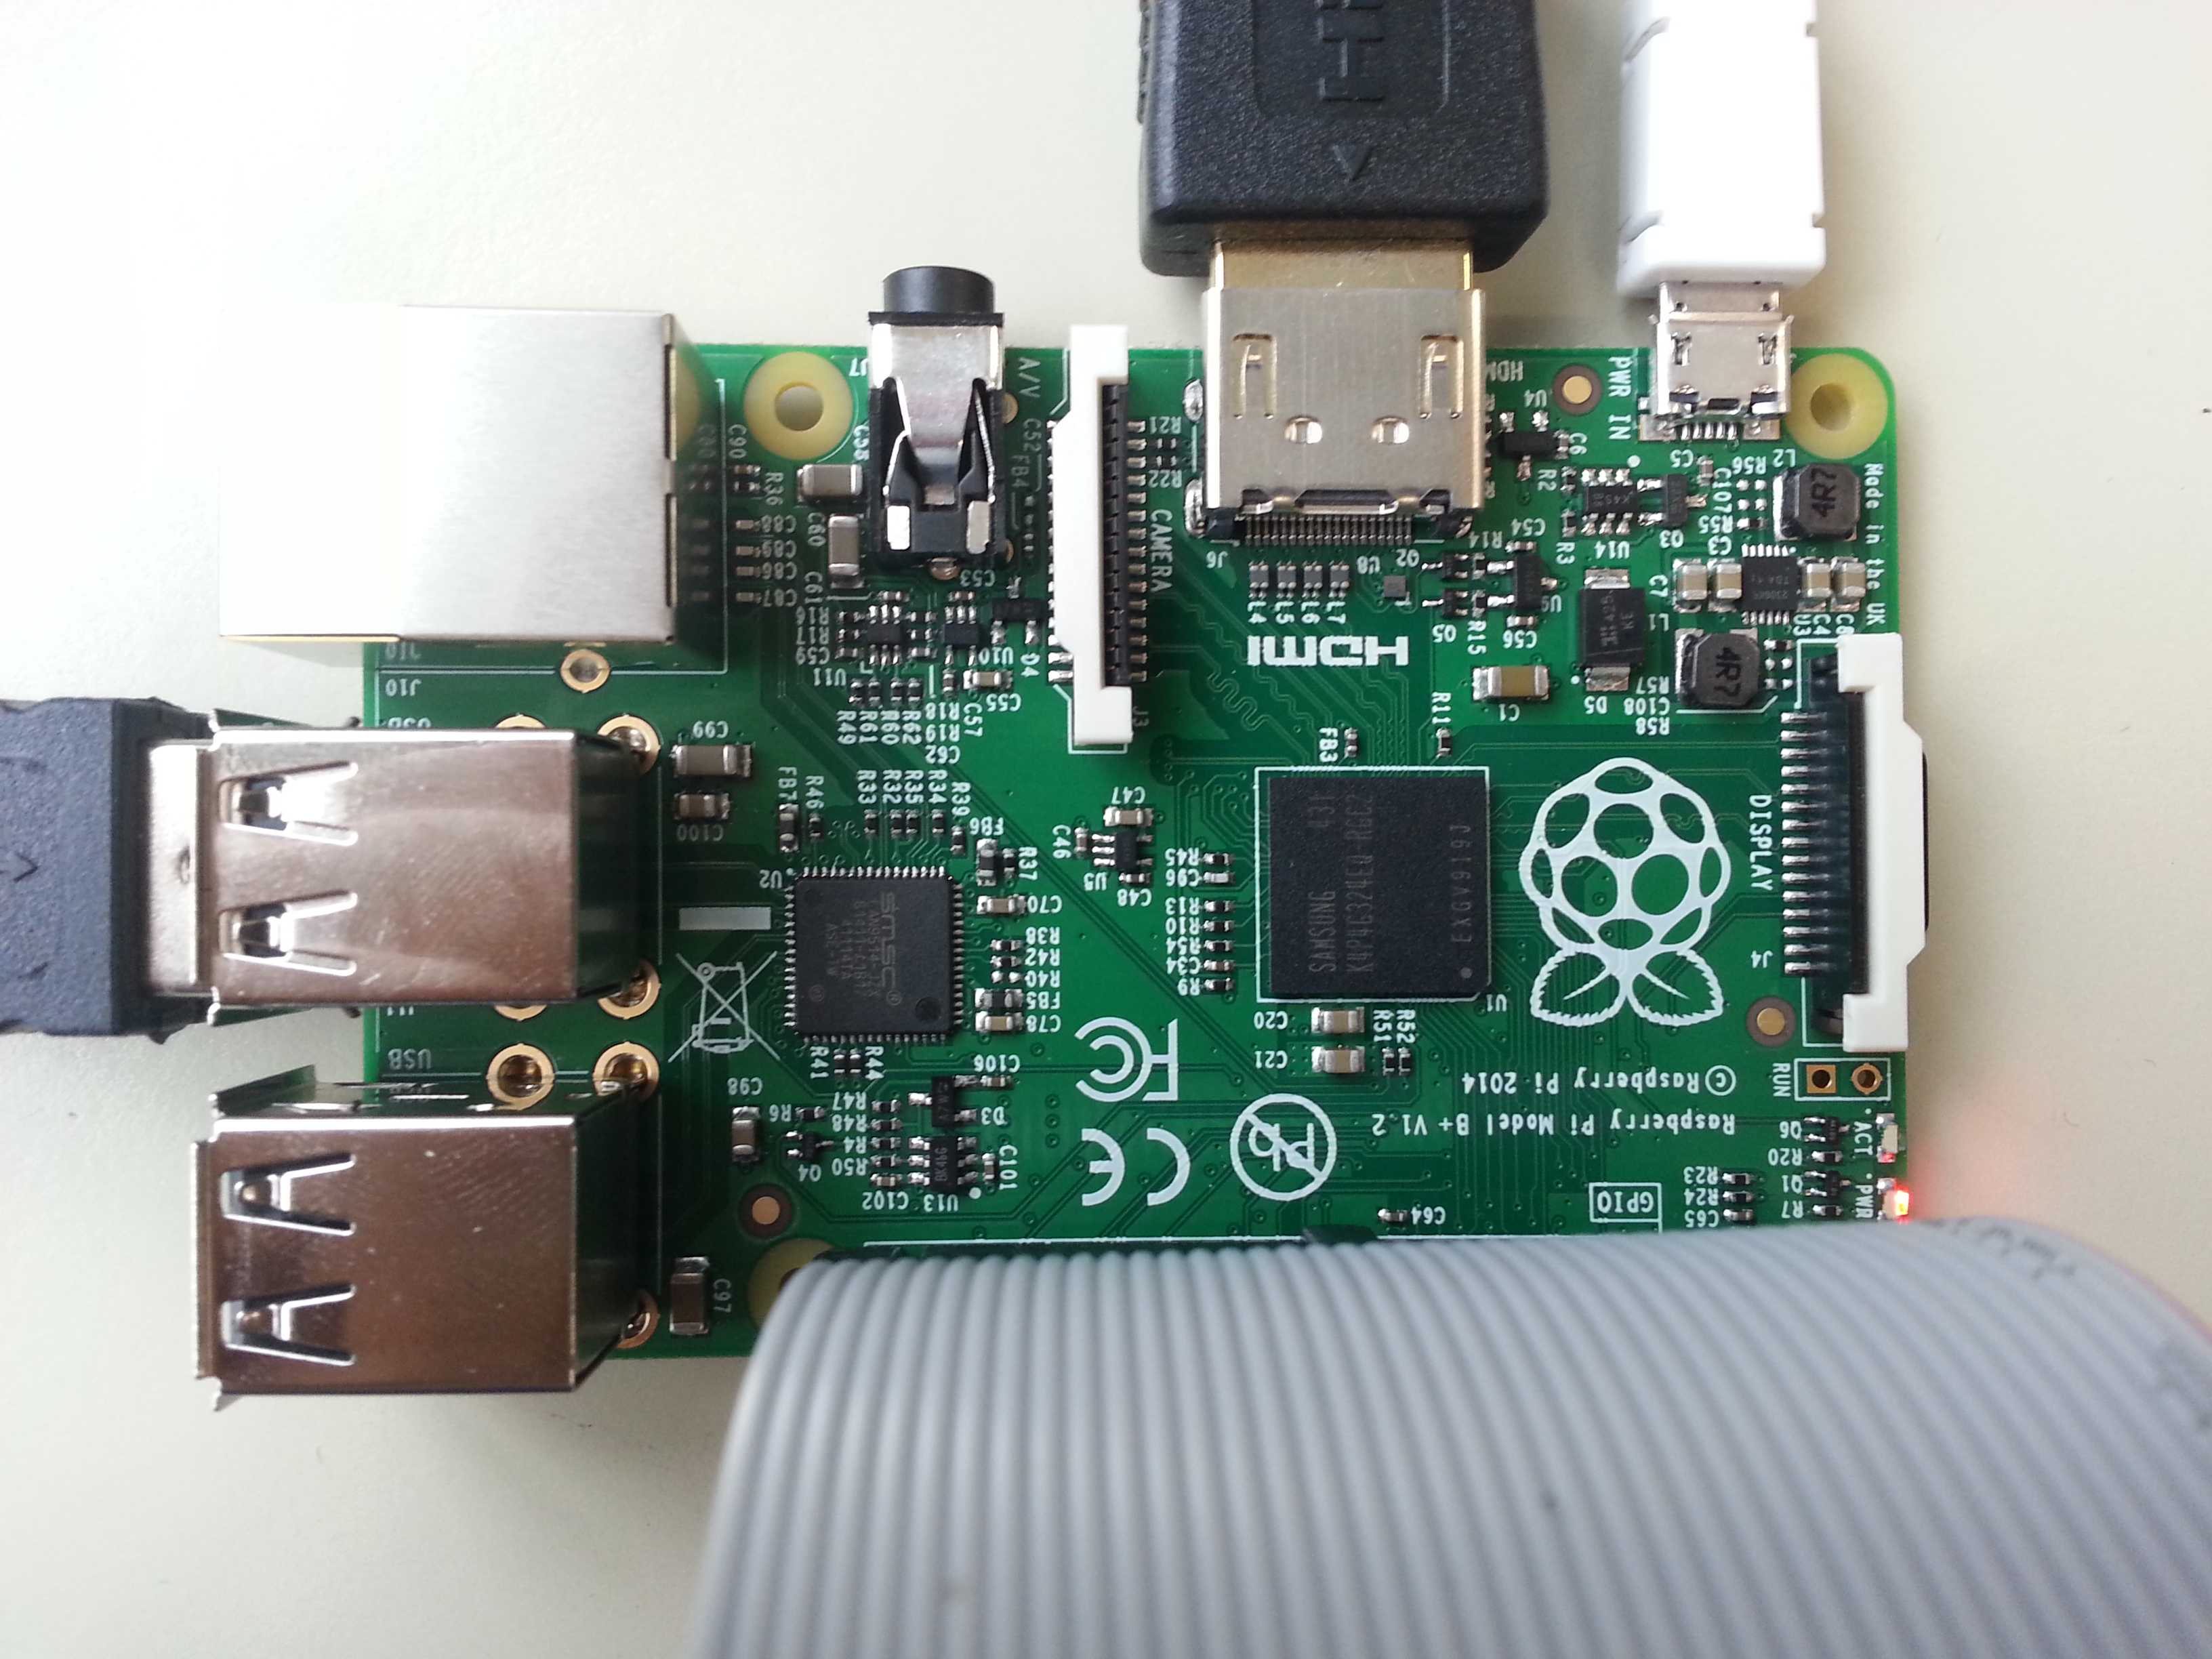
\includegraphics[width=\textwidth]{Test_unitaire/Rpi/img5.jpg}
\captionof{figure}{Notre Raspberry Pi B+}

~\\
\parindent=15pt

Pour s'assurer que notre Raspberry Pi répond aux spécifications fonctionnelles et qu'il fonctionne correctement en toutes circonstances pour notre projet, nous y avons réalisé des tests unitaires.

Après avoir enfin installé le système d'exploitation Raspbian\footnote{La documentation lié à Raspbian est situé en annexe à la page \pageref{annexe:raspbian}} sur notre Raspberry Pi B+, nous avons tenté de tester les ports GPIO. Pour cela, dans un premier temps, nous avons allumé des LED grâce à un script python à travers différents ports GPIO. Sur la figure \ref{figure:led}, on peut observer que nous avons allumé une LED grâce au port 22.
~\\

Dans notre projet le Raspberry Pi sera placé entre le radio-goniomètre à effet Doppler et l'utilisateur. Il aura deux taches, corréler les données entre tous les dispositifs pour obtenir la position du drone et afficher le résultat à l'utilisateur. Pour cela il doit récupérer la direction qui est donné par le Montréal 3v2. Cette position est donnée à travers des LED (voir figure \ref{figure:ledMontreal}). Nous allons donc placer le Raspberry Pi au niveau des LED pour obtenir les informations délivré par le Montréal 3v2. % TODO : A FINIR

\begin{figure}[!h]
  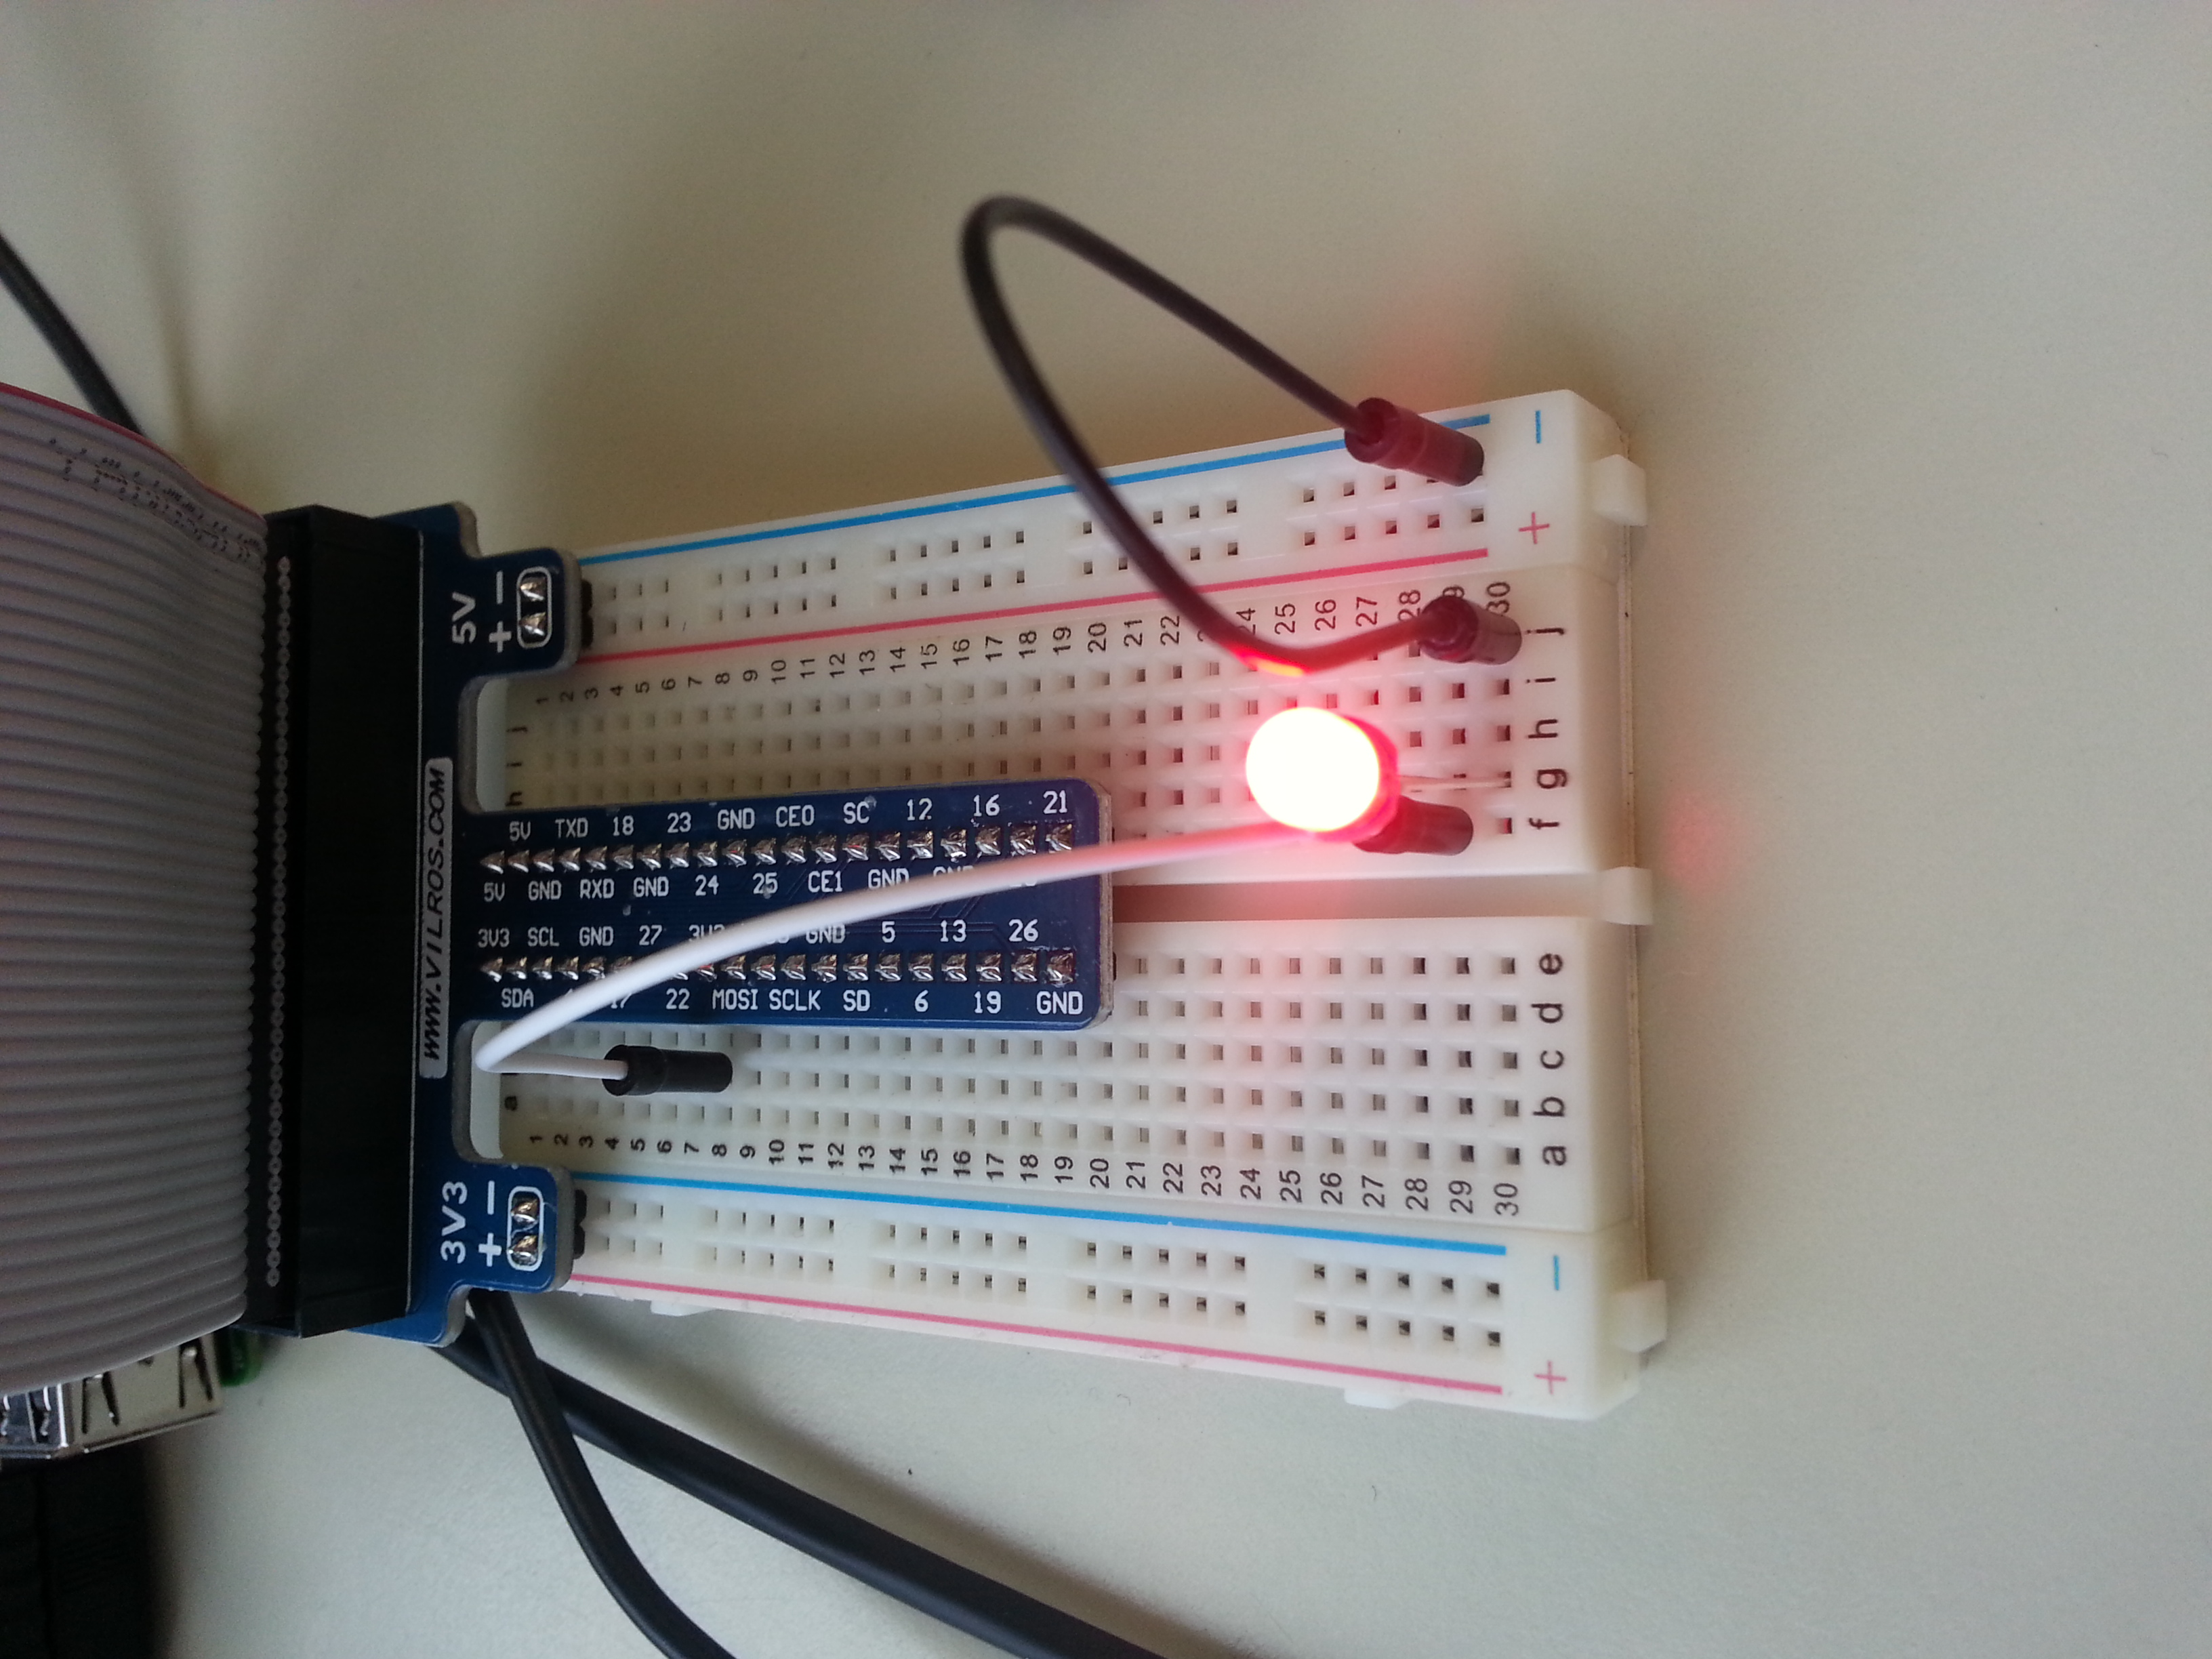
\includegraphics[width=\textwidth]{Test_unitaire/Rpi/img3.jpg}
  \caption{Allumage d'une LED par Raspberry Pi}
  \label{figure:led}
\end{figure}

\begin{figure}[!h]
  \centering
  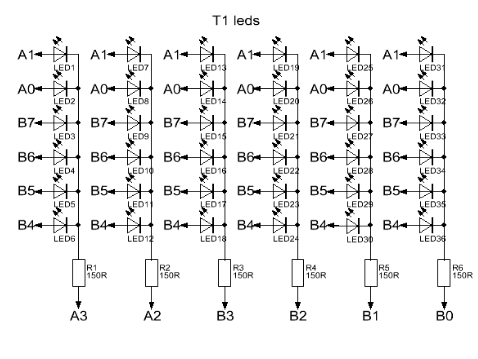
\includegraphics[width=0.8\textwidth]{Test_unitaire/Rpi/led.png}
  \caption{Méthode de connexion des leds dans le Montréal}  
  \label{figure:ledMontreal}
\end{figure}
\begin{figure}[!h]
  \centering
  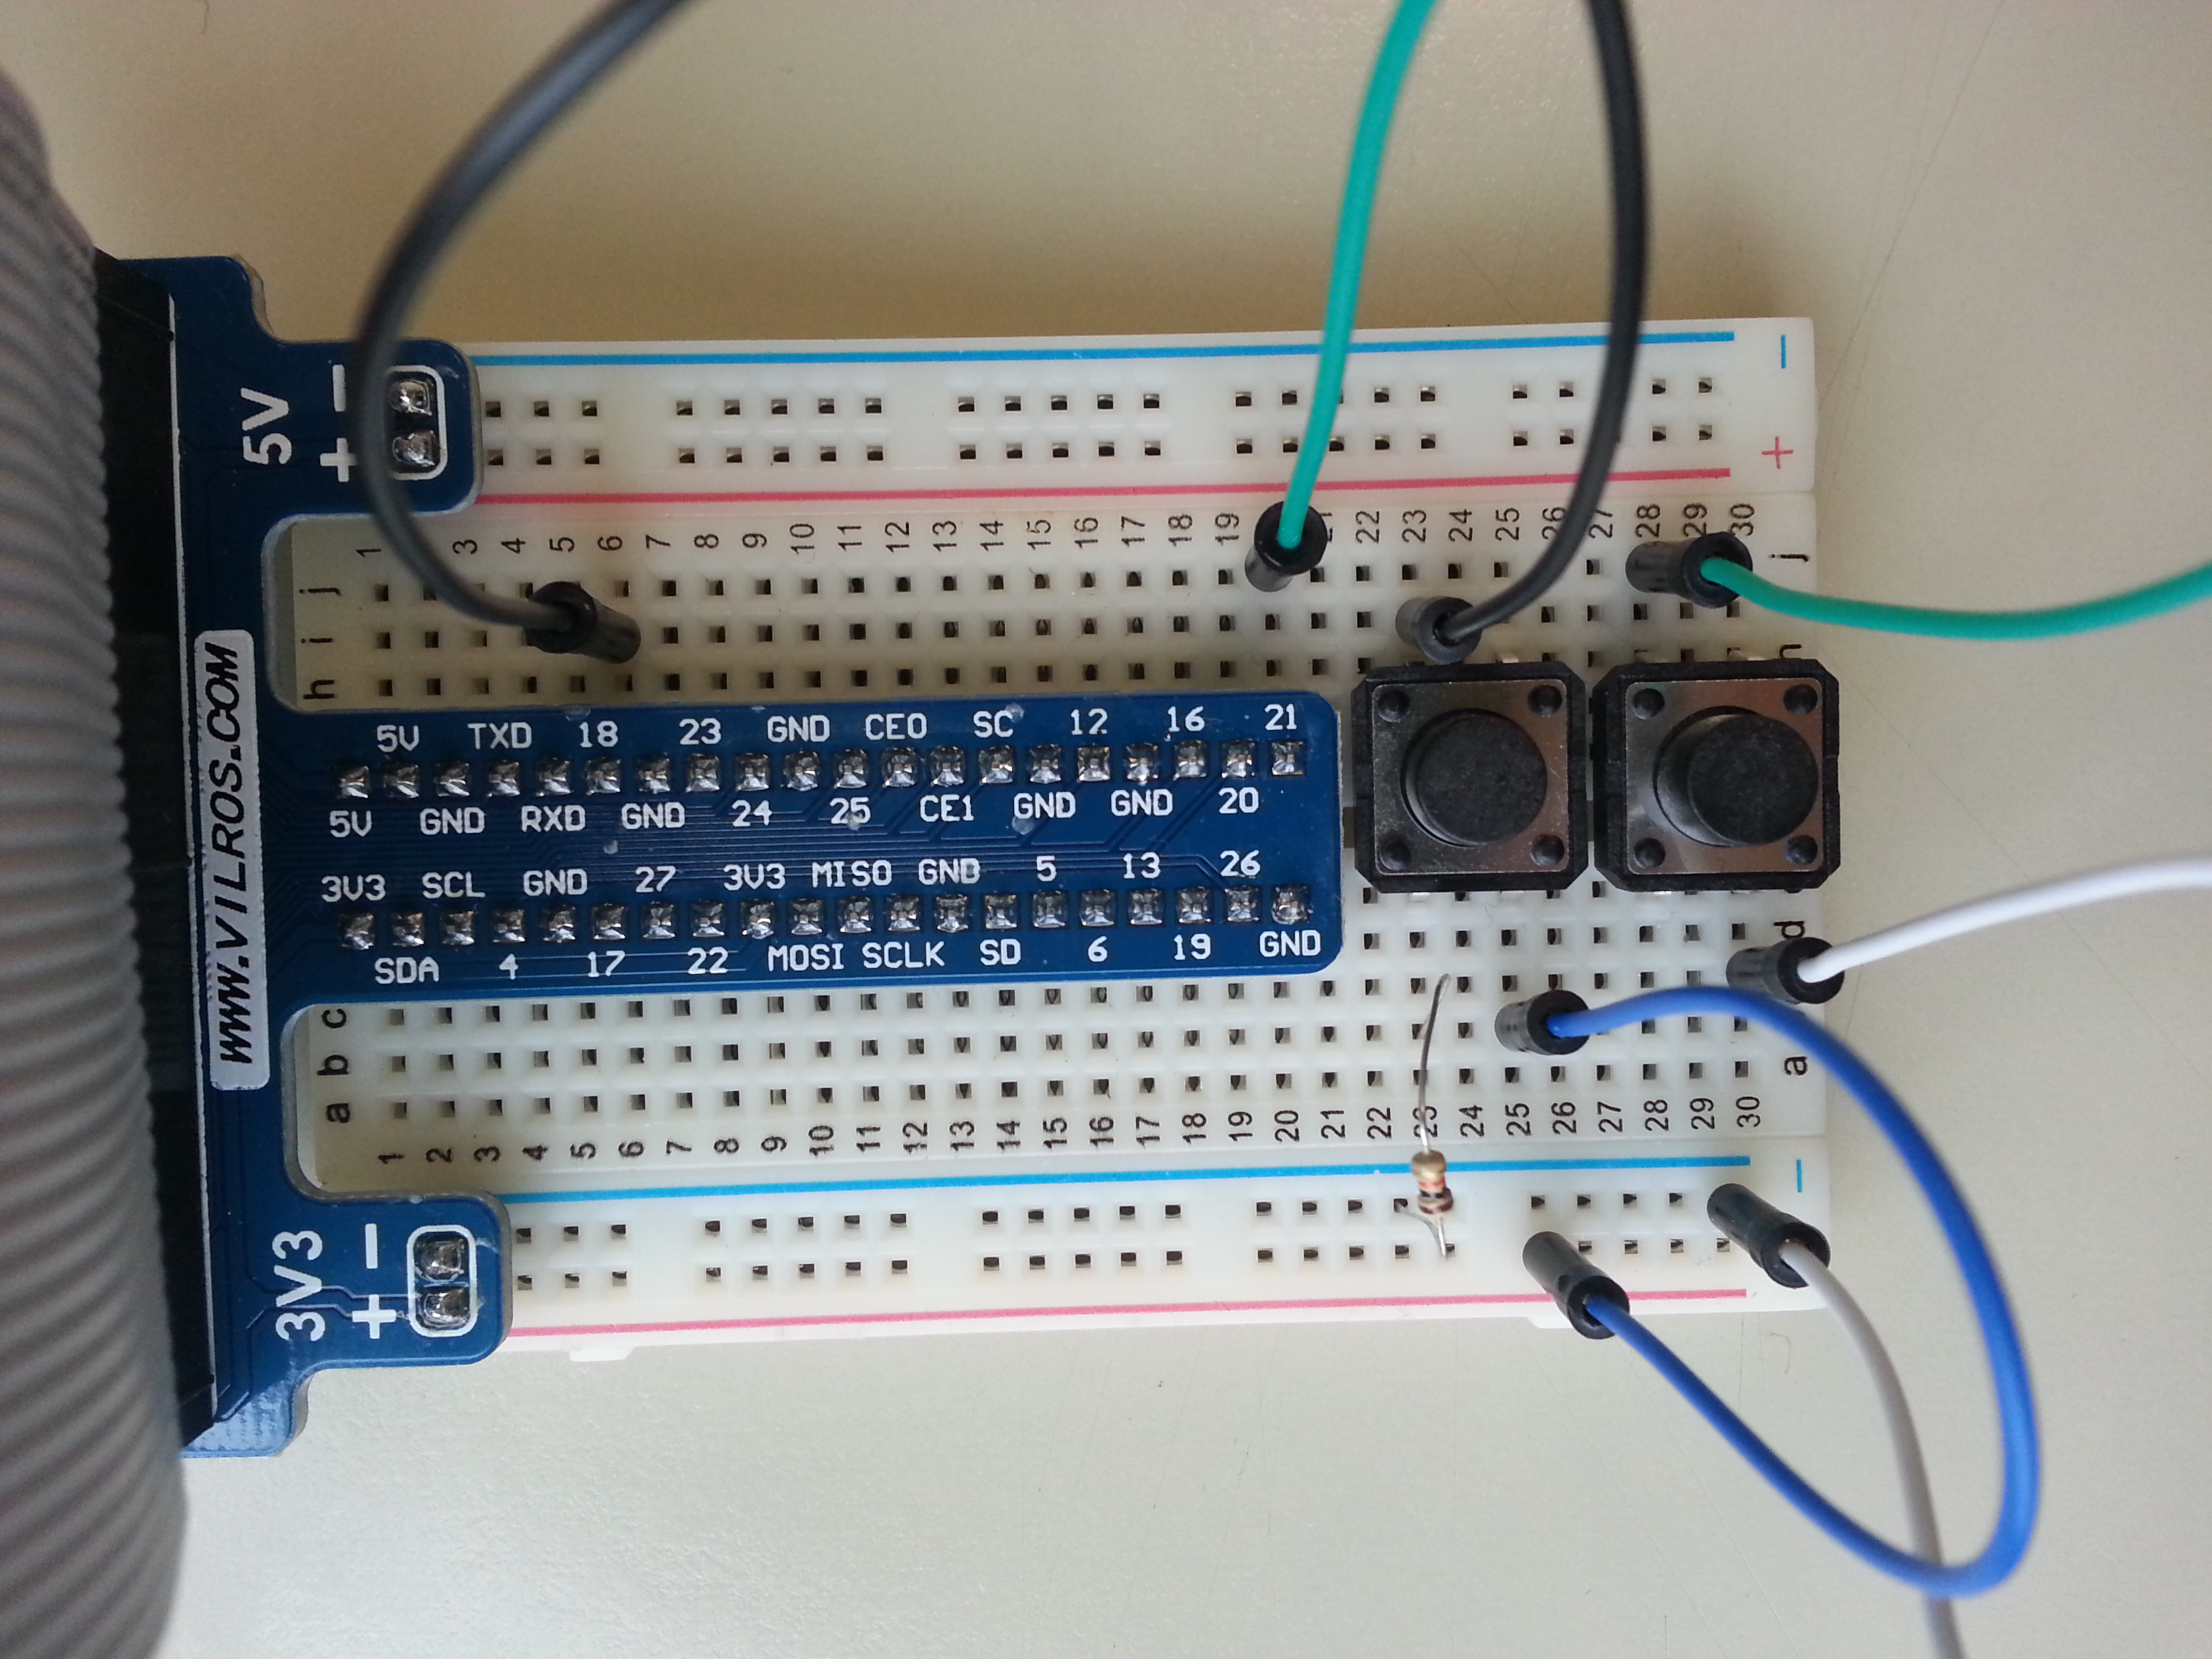
\includegraphics[width=\textwidth]{Test_unitaire/Rpi/img4.jpg}  
  \caption{Système modélisant une LED}
  \label{figure:test}
\end{figure}

La sortie du Montréal 3v2 est décrite à la figure \ref{figure:ledMontreal}. On constate que le pic qui permet l'affichage à 12 sortie qui lui permet de gérer 24 LED. Pour connaître quelle LED est allumé, il faut savoir laquelle des entré A1,A0,B7,B6,B5,B4 à un front montant et laquelle des entrées B0,B1,B2,B3,A3,A2 à un front descendant.

Pour modéliser une LED en entré du Raspberry Pi, nous avons positionné 2 boutons poussoirs (voir figure \ref{figure:test}). Le premier permets de réaliser le front montant et le second le front descendant. Ainsi en positionnant ces boutons au bon endroit par rapport au port GPIO du raspberry il est possible de connaître quelle LED on a simuler.

Nous avons réaliser un script python qui lié les entrées du raspberry avec les sortie du pic. Puis nous avons tester en simulant une LED comme décrit précédemment.

On peut constater que l'expérience est un succès car le raspberry pi nous renvoie bien le numéro de la LED que nous voulions tester.




%%%%%%%%%%%%%%%%%%%%%%%%%%%%%%%%%%%%%%%%%%%%%%%%%%%

\section{PIC}
\label{sec:pic}

Dans le schéma du Montréal 3v2 nous avons pu constater qu'il y avait 3 PIC programmés. Nous avons commandé les PIC programmés au près de l'entreprise F1LVT \cite{montreal}.


\begin{figure}[!h]
  \centering
  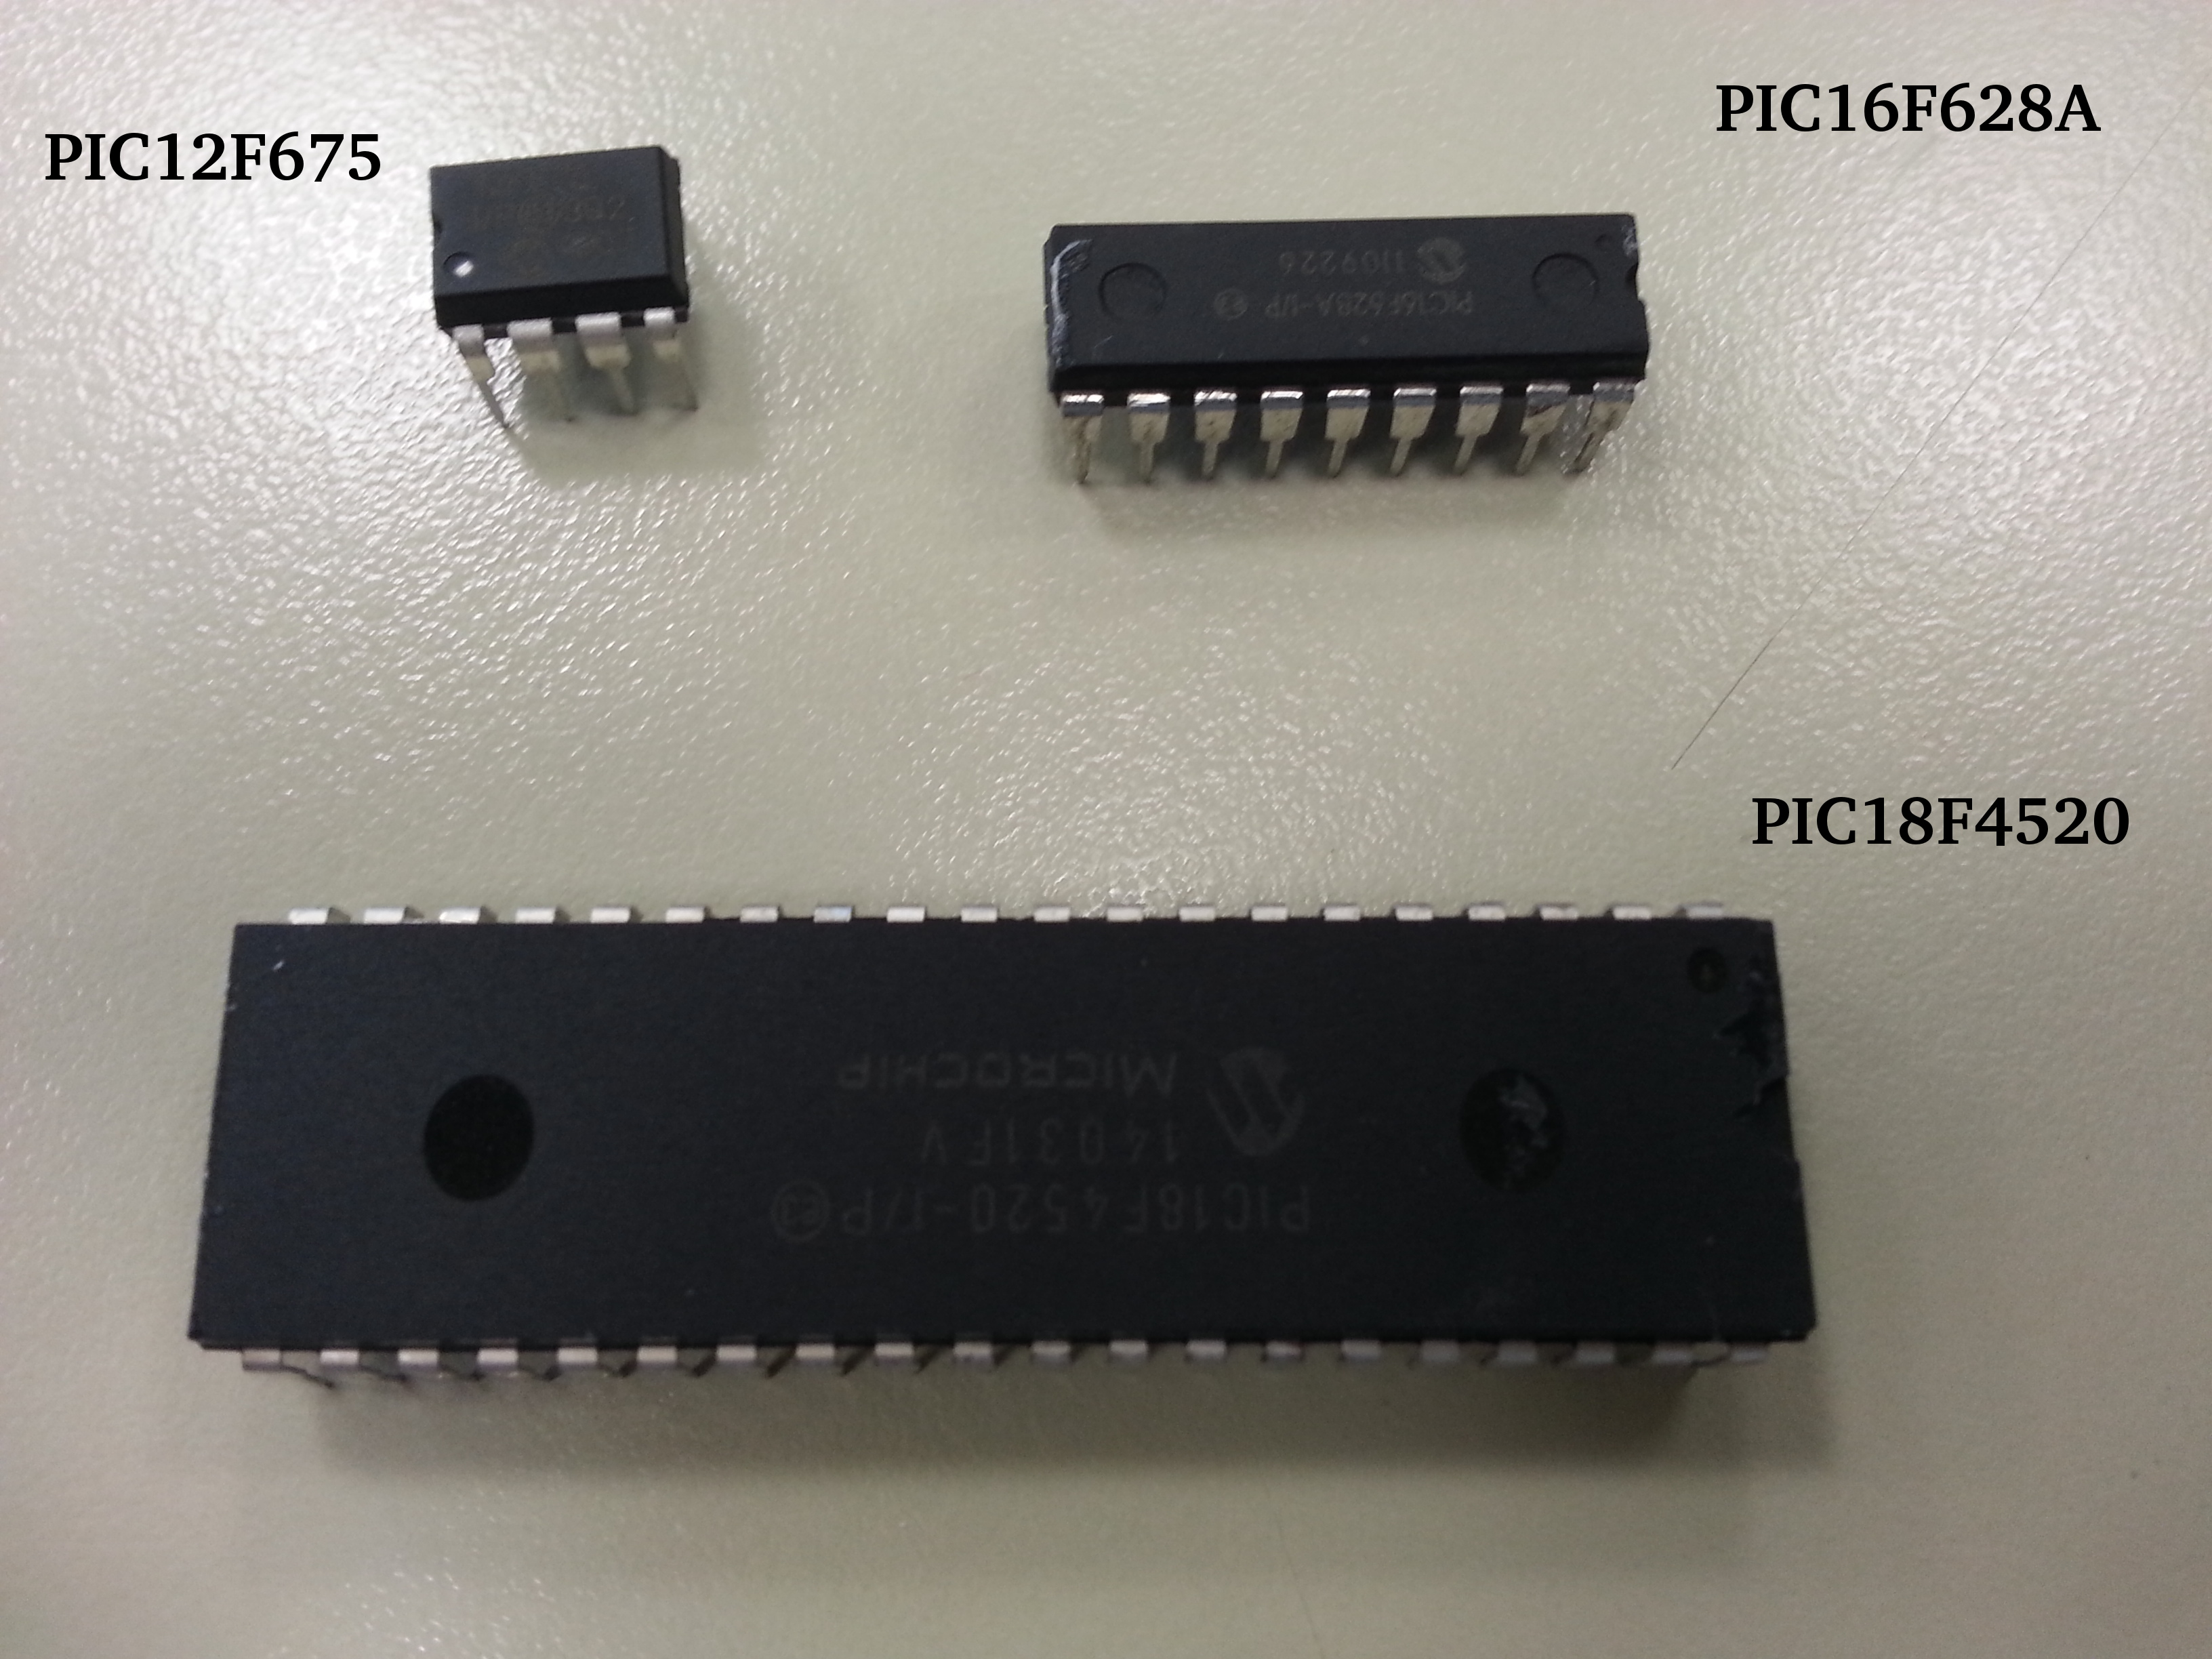
\includegraphics[width=\textwidth]{Test_unitaire/Pic/pic}
  \caption{3 PIC programmés}
  \label{fig:pic}
\end{figure}

Nous avons ensuite imaginé et réalisé des tests unitaires sur chacun des PIC pour vérifier qu'ils ont bien été programmés et qu'aucune erreur n'est apparu sur ce système de décision critique pour le système.

\subsection{PIC16F628A}
\label{sec:picled}

Ce PIC sert à réaliser l'affichage sur les LED. Pour tester ce PIC, nous avons réaliser le montage de la figure \ref{fig:picled}. On peut voir à la figure \ref{fig:schemapic} le schéma de montage du PIC sur le Montréal 3v2.

\begin{figure}[!h]
  \centering
  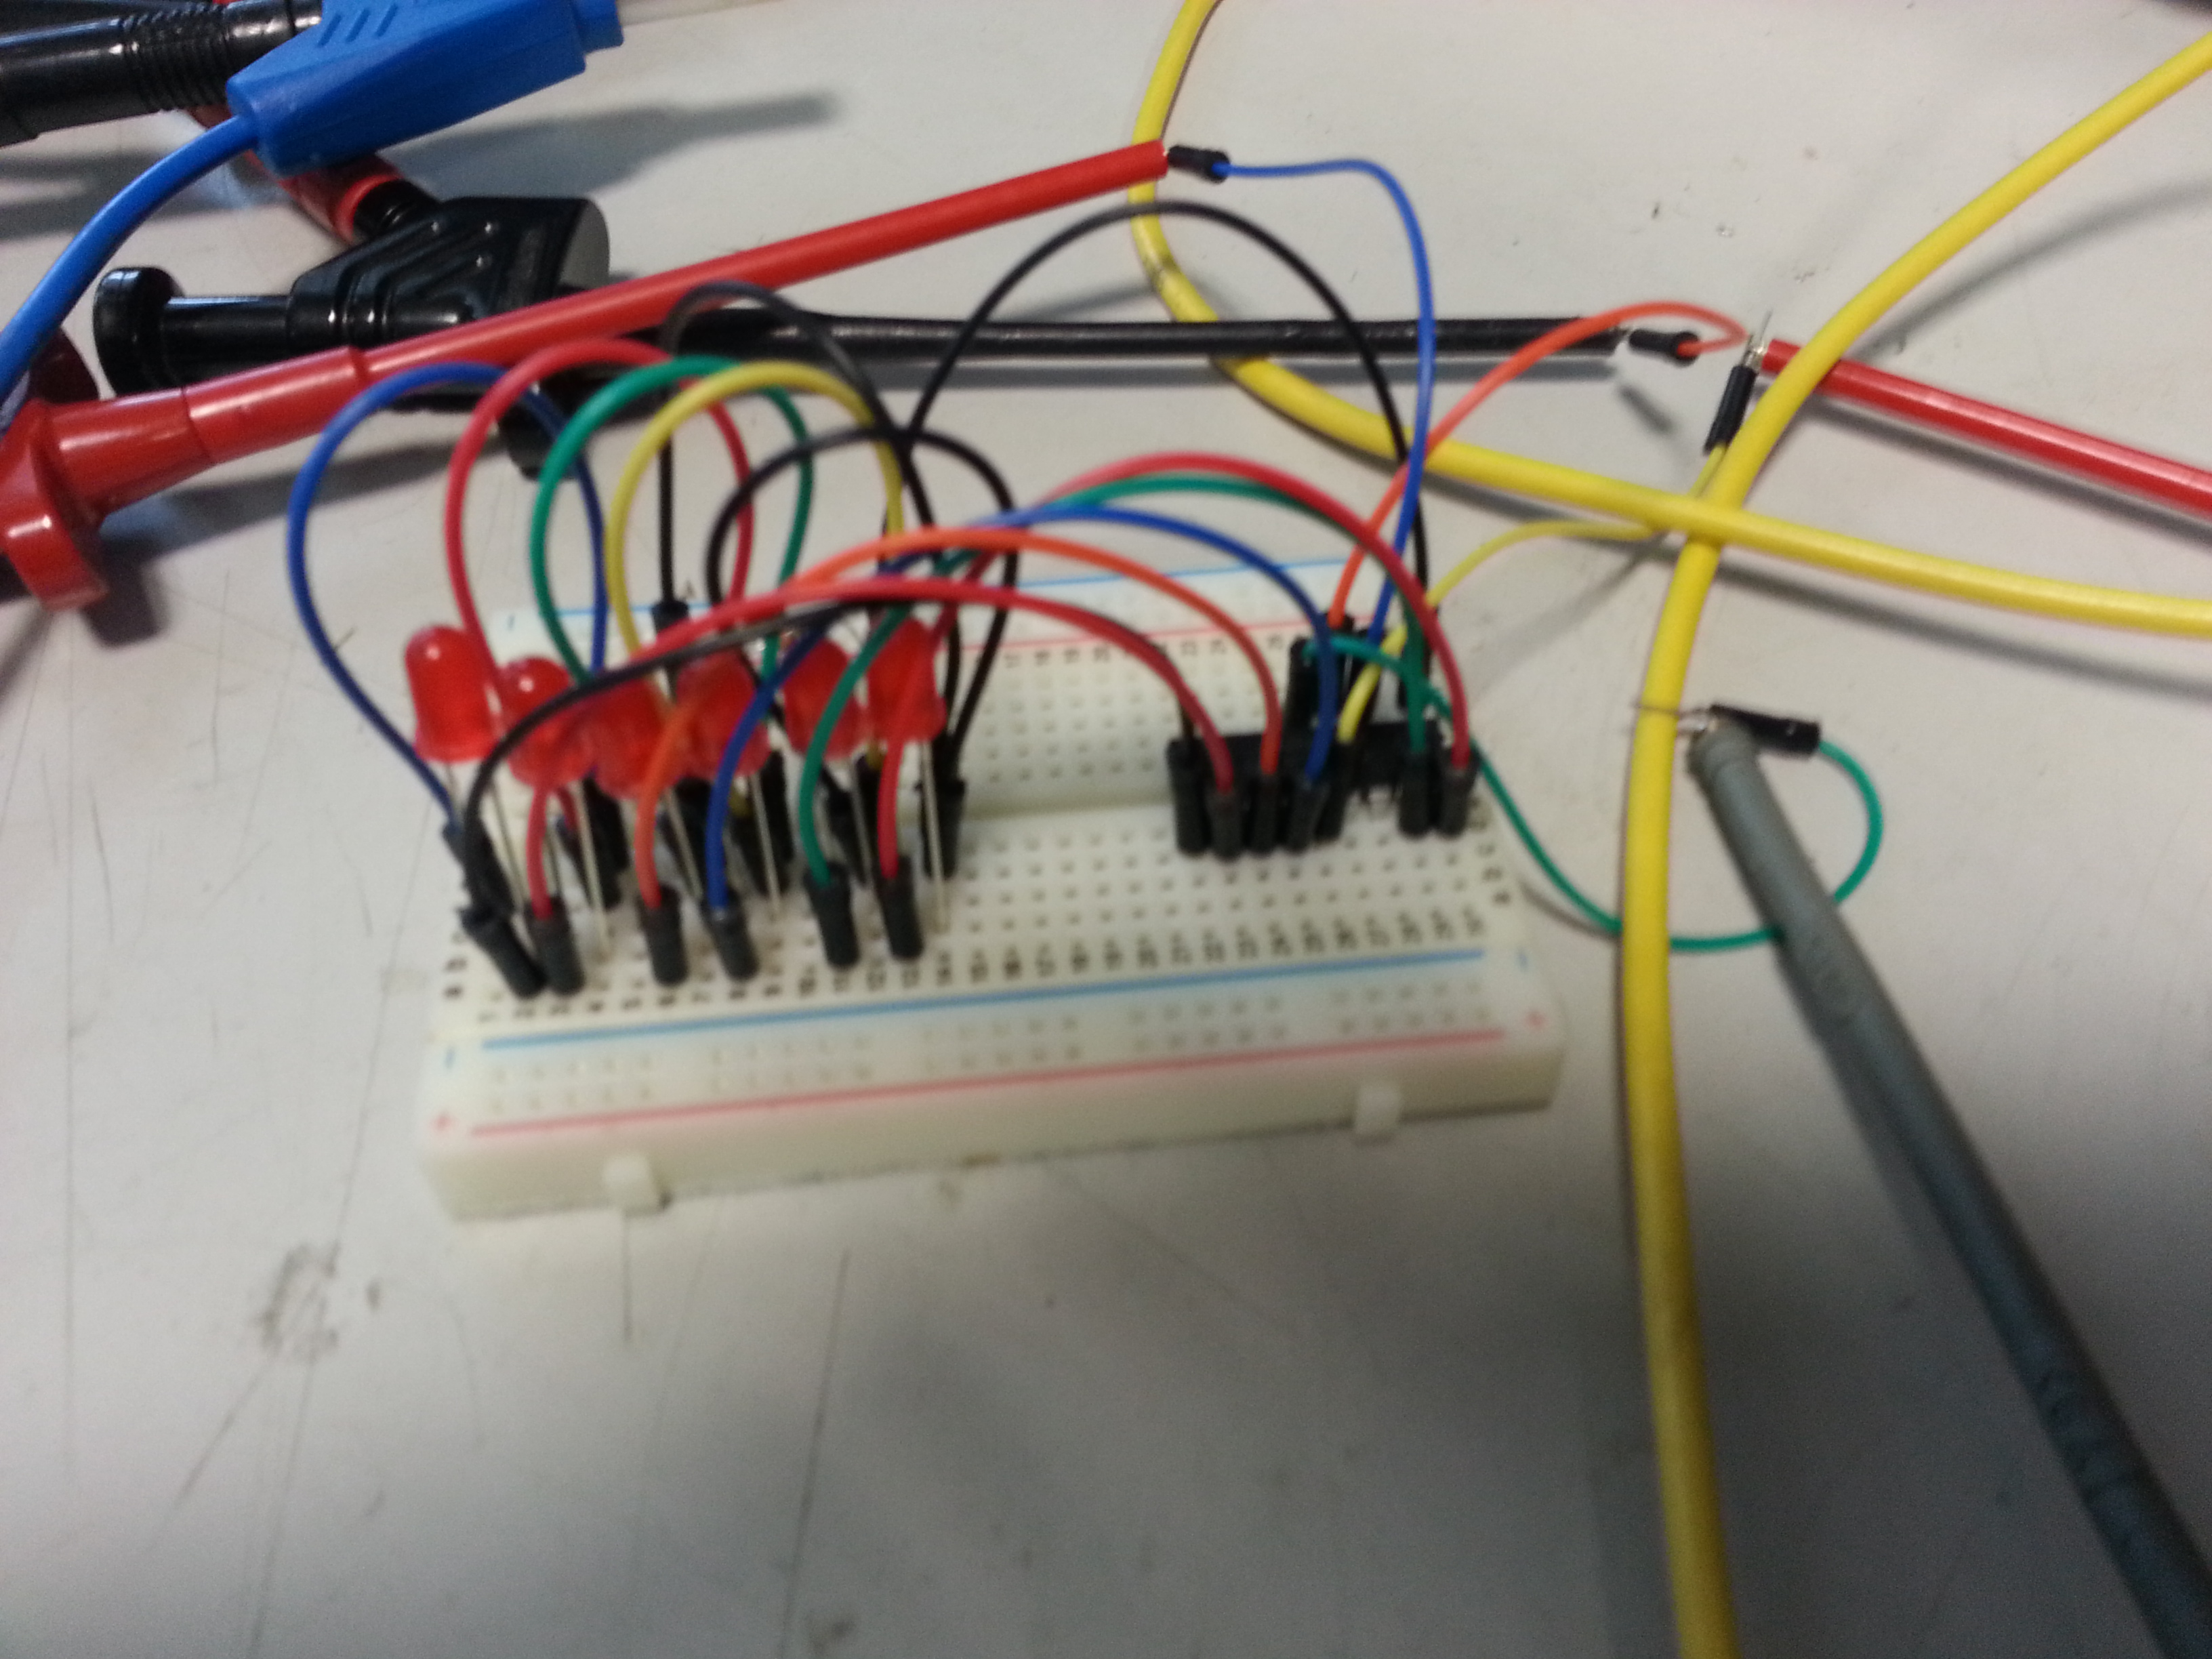
\includegraphics[width=\textwidth]{Test_unitaire/Pic/picled}
  \caption{Schéma electrique du test unitaire}
  \label{fig:picled}
\end{figure}


Pour tester ce composant, nous avons donc choisi de monter une partie des LED situés en sorti, de configurer le \og clock\fg{} sur un signal carré de fréquence 1 MHz, et de faire varier la fréquence de l'entrée \og data\fg{}.

Malheureusement nous n'avons pas pu observer de LED s'allumer pendant notre expérience.

\begin{figure}[!h]
  \centering
  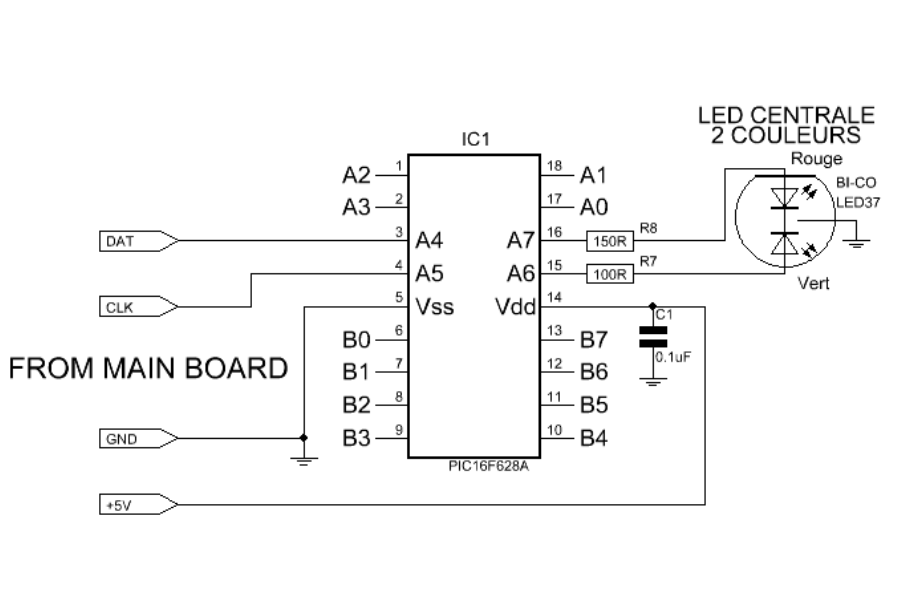
\includegraphics[width=\textwidth]{Test_unitaire/Pic/schemapic}
  \caption{Schéma de montage du pic sur le Montréal 3v2}
  \label{fig:schemapic}
\end{figure}
\newpage
\subsection{PIC12F675}
\label{sec:picclock}

\subsection{PIC18F4520}
\label{sec:piccontrol}


\section{Filtre passe bande}
\label{sec:passe_bande}


Pour le filtre passe bande, nous souhaitions un filtre qui couperait tout ce qui se trouve en dehors de notre bande, au final ce filtre réagit plutôt bien quand le montage qui y est lié est adapté, ce qui est le cas, le circuit fonctionne bien a 50 Ohm.

Le test unitaire était simple on a branché le filtre sur un analyseur que envoyais un signal et recevait ce même message. Il est alors simple d’obtenir le comportement du filtre. Nous avons obtenu que le filtre diminuait très bien ce que ce trouve avant 2.4GHz mais plutôt mal ce qui vient après. Mais ceci n’est pas gênant car les bande entre 205Ghz et 5 GHz ne sont pas ou peu utilisé en France.

\begin{figure}[h]
  \centering
  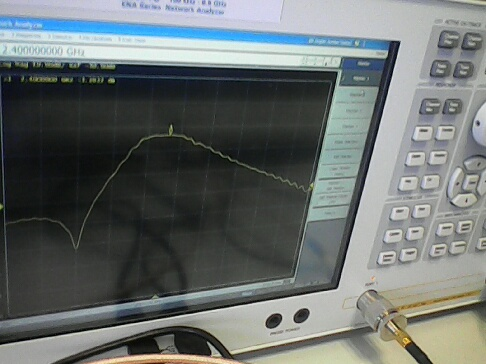
\includegraphics[width=0.8\textwidth]{oscillo1}
  \caption{Comportement du filtre}
  \label{fig:comportement}
\end{figure}

Sur la photo le curseur sur la courbe est à 2.45Ghz et le plat est un peu plus grand que la bande.

Nous avons mesuré deux paramètres supplémentaires, Le S11 et le S21 qui sont des paramètres permettant de mesurer la perte d’amplitude. Le S11 est le coefficient de réflexion à l'entrée lorsque la sortie est adaptée. Dans l’idéal il vaut 0, il n’y a alors aucune réflexion et tout l’amplitude du signal sort du filtre, on obtient le S11 de la photo suivante.

On peut voir ici que le log du S11 est très faible entre 2.4 et 2.5 GHz ce qui est bon pour le filtre.

\begin{figure}[h]
  \centering
  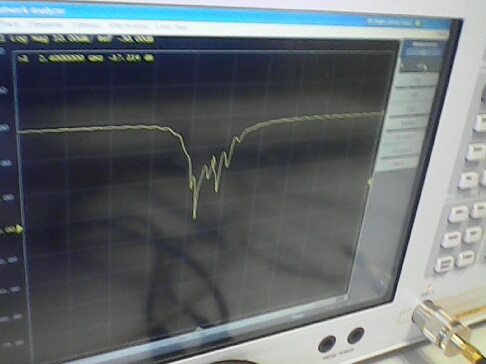
\includegraphics[width=0.8\textwidth]{oscillo2}
  \caption{S11 du filtre passe bande}
  \label{fig:filtre}
\end{figure}


Les deux plus grands pics vers le bas correspondent aux limites de la bande 2.4-2.5GHz.

Le S21 est le coefficient de transmission direct lorsque la sortie est adaptée, pour celui-ci le but est d’avoir ce nombre le plus proche de 1 et donc son logarithme le plus proche de zéro possible.

Lors du test, nous avions une perte d’environ 2dBm dans la bande de fréquence 2.4-2.5GHz, ce qui est peu, le filtre ne risque donc pas d’occulté ce que l’on souhaite voir.
\newpage
\section{VCO}



Le test du VCO est simple mais doit être bien fait car sans lui impossible d’obtenir la bonne fréquence à la fin.

Nous avons commencé par mesurer la fréquence libre, c’est-à-dire la fréquence renvoyée par le VCO s’il est juste alimenté et que la tension d’entrée est nulle. La fréquence libre qui était de 1.35 GHz était plus grande que la fréquence indiqué par le constructeur (1.31Ghz) ensuite nous avons mesuré la tension pour laquelle nous obtenions 1.9Ghz et nous avons obtenu environ 8V ce qui nous à permit de choisir le bon régulateur de tension pour la suite. Les régulateur sont calibrés, il est donc difficile d’en trouver un qui corresponde parfaitement mais on a pu obtenir un régulateur à 8.1V ce qui après test donnait 1.91GHz. La bande de fréquence a transférer étant de 100 MHz nous n’étions pas à 10 MHz prés et il aurait été difficile et couteux de trouver un meilleur moyen de le faire.


\begin{figure}[h]
  \centering
  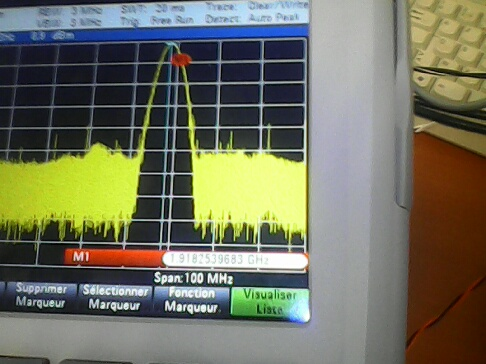
\includegraphics[width=0.8\textwidth]{oscillo3}
  \caption{Fréquences généré par le VCO alimenté à 8.1V centrée autour de 1.9GHz d’une largeur d’environ 10MHz}
  \label{fig:freq}
\end{figure}
\newpage
\section{Down converter}
\label{sec:down_converter}



\begin{figure}[h]
  \centering
  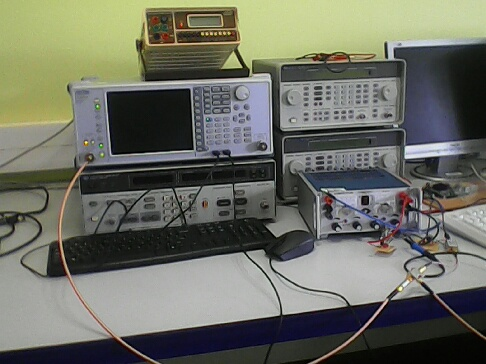
\includegraphics[width=0.8\textwidth]{oscillo4}
  \caption{Montage de test de l’adaptateur}
  \label{fig:mont}
\end{figure}


Le test du down converteur a posé certain problème. En effet le seul moyen de le tester est de le tester dans son cas d’utilisation pratique. Il est, en effet, nécessaire de l’alimenter et  ceci ne peut se faire sans le VCO, de même le bruit risque de gêner l’observation, il faut donc utiliser le filtre.


\begin{figure}[h]
  \centering
  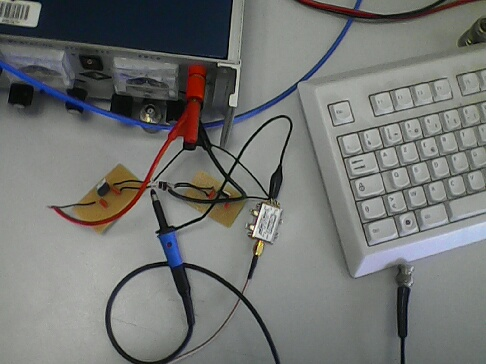
\includegraphics[width=0.8\textwidth]{oscillo5}
  \caption{Photo du VCO et de son alimentation}
  \label{fig:photo}
\end{figure}



Nous avons rencontré des problèmes lors du test, premièrement, des problèmes de communication entre membre de l’équipe ont retardé le test d’une semaine, en effet il a fallu crée un montage avec les deux régulateurs de tension, celui pour l’alimentation et celui pour la tension en entrée. Le premier membre de l’équipe a demandé au second de souder le montage mais n’a pas présenté l’ordre dans lequel il devait être placé ce qui a entrainé une inversion. Ceci a retardé la phase de test

Deuxièmement, nous n’avions pas prévue les problèmes dus aux câbles. Il a fallu en effet cherché des câbles en n’étant pas certain que le câblage utilisé ne ferait pas griller le matériel.

Troisièmement, le professeur nous ayant aidé lors de la conception théorique du montage était en déplacement, il n’a donc pas pu nous aider lorsque des hésitations se sont fait sentir, devant le prix du matériel et la possibilité de le griller, nous n’avons pas pu le faire fonctionner.

Enfin, par manque de temps, nous n’avons pas eu l’occasion de refaire ce test.




%%% Local Variables: 
%%% mode: latex
%%% TeX-master: "../rapport"
%%% End: 
